\documentclass[hidelinks]{ctexart}

\usepackage[sensei=陈向军/刘明辉,gakka=原子物理学,section=Kiso,gakkabbr=AP]{styles/kurisu}
\usepackage{van-de-la-illinoise}
\usepackage{van-le-trompe-loeil}

\begin{document}

\section{原子模型和单电子原子} % (fold)
\label{sec:原子模型和单电子原子}

\noindent\textbf{配置}\\[.5em]
\noindent
Chen Xiangjun, xjun@ustc.edu.cn \\
Liu Minghui, hepglmh@ustd.edu.cn \\
T.A. Chen Guangqing, CGQ1113@mail.ustc.edu.cn \\
T.A. Li Yue, ly60@mail.ustc.edu.cn \\
905881973\\
作业(25\%)+5次小测(5\%)+研讨课(10\%)+期末(60\%), 研讨课W5, W7, W9, W11, W13, W15六次.\\
研讨课上Doodle注册.

\subsection{物质的原子性} % (fold)
\label{sub:物质的原子性}

$\SI{12}{\gram}$的$\ce{^{12}C}$为$\SI{1}{\mole}$. 对应粒子数
\[ N_A = \SI{6.02214086e23}{\per\mol}. \]
$\ce{^{12}C}$原子质量的$1/12$为$1$原子单位,
\[ \SI{1}{\atomicmass} = \SI{1.67e-27}{\kilo\gram}. \]
原子数密度
\[ N = \frac{\rho}{A}N_A. \]
\begin{ex}
    对于固体铜,
    \[ N = \frac{\SI{8.69}{\gram\per\cubic\centi\meter}}{63.5}\times 6.022\times 10^{23} = \SI{8.49e22}{\per\cubic\centi\meter}. \]
\end{ex}
原子的大小可以估计为
\[ V_A = \rec{N} = \frac{A}{\rho N_A}. \]
对于球形密堆积,
\[ V_A = 4\sqrt{2}R^3,\quad R = \pare{\frac{A}{4\sqrt{2}\rho N_A}}^{1/3}. \]
\begin{remark}
    不同元素的原子半径差异不大. 皆在$\SI{}{\angstrom}$量级.
\end{remark}

% subsection 物质的原子性 (end)

\subsection{电子} % (fold)
\label{sub:电子}

\subsubsection{电子的发现} % (fold)
\label{ssub:电子的发现}

电子的发现源于阴极射线. J.J. Thomson的实验表明阴极射线的速度$\SI{1.9e5}{\meter\per\second}\ll c$, 且通过磁场证实其带负电.
\par
电解单价离子, 则$A\leftrightarrow F = \SI{96484.6}{\coulomb}$. 故$e = F/N_A$.
\par
混合电场和磁场, $\+vE + \+vv\times\+vB = 0$, 可测得荷质比, 此时
\[ \frac{qE}{m}\frac{l}{v_p} = \frac{qlB}{m}. \]
从而, 若设仅有电场时偏转量为$h$, 则
\[ \frac{h}{L} = \frac{v_\perp}{v_p} = \frac{qlB}{m}/\frac{E}{B} = \frac{qlB^2}{mE}\Rightarrow \frac{q}{m} = \frac{hE}{lLB^2}, \]
其中$l$为磁场区域范围, $L$为运动总长度. 其荷质比与离子相去甚远. 射线可穿过铝箔, 故并非带点量大的离子.
\par
Millikan油滴实验中, 设液滴半径$r$, 密度$\rho$, 空气密度$\rho_0$, 粘滞系数$\eta$. 则不加电压时,
\[ \frac{4}{3}\pi r^3\rho g = 6\pi \eta rv_g + \frac{4}{3}r^3\rho_0 g \Rightarrow 4\pi\eta rv_g = \frac{4}{3} \pi r^3 \pare{\rho - \rho_0}g. \]
测量收尾速度后得到
\[ \resumath{r = \sqrt{\frac{9\eta v_g}{2\pare{\rho - \rho_0}g}}.} \]
设油滴带负电荷$e_k$, 电容器上加电压$+V$, 电容版间距$l$, 油滴在电场力作用下会掉头向上运动.
\[ F_e = e_k \frac{V}{l}. \]
平衡时收尾速度满足
\[ \frac{4}{3}\pi r^3\rho_0 g + e_k \frac{V}{l} = 4\pi\eta rv_e + \frac{4}{3}\pi r^3 \rho g. \]
测量收尾速度, 则
\[ \resumath{e_k = \frac{l}{V}\brac{4\pi \eta r v_e + \frac{4}{3}\pi r^3\pare{\rho - \rho_0}g} = \frac{6\pi \eta rl}{V}\pare{v_e + v_g}.} \]
\begin{remark}
    采用数值$\resumath{\displaystyle \frac{e^2}{4\pi\epsilon_0} = \SI{1.44}{\eV\cdot\nano\meter}, m_ec^2 = \SI{0.511}{\mega\eV}.}$
\end{remark}

% subsubsection 电子的发现 (end)

\subsubsection{Thomson原子模型} % (fold)
\label{ssub:thomson原子模型}

这一模型要求原子中带正电的物质的量约等于全部的原子质量, 电荷量$+Ze$. 即Plum-Pudding模型. 可以解释原子的电中性, 稳定性, 并定型解释辐射特性.

% subsubsection thomson原子模型 (end)

% subsection 电子 (end)

\subsection{Rutherford原子模型} % (fold)
\label{sub:rutherford原子模型}

\mathsubsubsection{AlphaSc}{$\alpha$粒子散射...}{$\alpha$粒子散射实验}{Alpha粒子散射实验} % (fold)
\label{ssub:alpha粒子散射实验}

放射性元素矿的衰变可以产生$\alpha$粒子, 电子和光子. $\alpha$粒子即\ce{He^{2+}}, 质量$m_\alpha \approx 4m_H$, 带电$q=2e$.
\par
$\alpha$粒子的对铂箔($\SI{}{\micro\meter}$厚度)的散射实验表明绝大$\alpha$粒子都直接穿透, 但大约$1/8000$的粒子的散射角大于$\SI{90}{\degree}$.
\begin{ex}
    设$\alpha$粒子入射能量$\SI{5}{\eV}$, 散射体厚度$\SI{1}{\micro\meter}$, 利用Thomson模型估计$\alpha$粒子的偏转角以及散射角度大于$\SI{90}{\degree}$的概率.
\end{ex}
\centerline{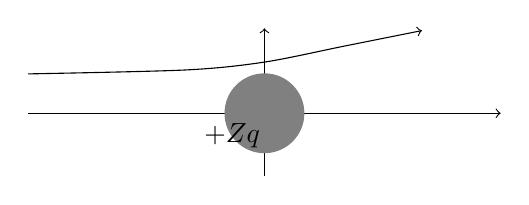
\begin{tikzpicture}
    \draw [->] plot [smooth] coordinates {(-3,0.5) (-1,0.55) (0,0.65) (1,0.85) (2,1.05)};
    \draw [->] (-3,0) -- (3,0);
    \draw [->] (0,-0.8) -- (0,1.08);
    \filldraw [gray] (0,0) circle (0.5);
    \draw (215:0.5) node {$+Zq$};
\end{tikzpicture}}
\begin{solution}
    由于$m_e \ll m_\alpha$, 忽略电子的影响. $\alpha$粒子受力
    \[ F_c = \left\{\begin{aligned}
        & \rec{4\pi\epsilon_0} \frac{2Ze^2}{r^2}, && r > R, \\
        & \rec{4\pi\epsilon_0} \frac{2Ze^2r}{R^3}, && r\le R.
    \end{aligned}\right. \Rightarrow F\+_max_ = \rec{4\pi\epsilon_0} \frac{2Ze^2}{R^2},\quad r=R. \]
    飞越时间大约为$R/v$, 故
    \[ \Delta p \sim \rec{4\pi\epsilon_0} \frac{2Ze^2}{R^2} \frac{R}{\sqrt{2E/m_\alpha}} = \rec{4\pi\epsilon_0} \frac{2Ze^2}{\sqrt{2E/m_\alpha}R}. \]
    由$\Delta p \sim p_0\theta_1$,
    \[ \theta_1 \sim \frac{\Delta p}{p} = \frac{e^2}{4\pi\epsilon_0}\frac{Z}{RE} = \SI{1.44}{\eV\cdot\nano\meter} \cdot \frac{78}{\SI{1}{\angstrom}\times\SI{5}{\mega\eV}} = \SI{2.2e-4}{\radian} = \SI{0.01}{\degree}. \]
    当大量$\alpha$粒子穿过铂箔, 散射角$\theta$随机分布, 有
    \[ f\pare{\theta}\,\rd{\theta} = \rec{\sqrt{2\pi\overbar{\theta}^2}}\exp\pare{-\frac{\theta^2}{\overbar{\theta}^2}}\,\rd{\theta}. \]
    其中$\overbar{\theta}$是散射角的方均值, $\overbar{\theta}^2 = N\overbar{\theta_1}^2$. 设$N\sim 10^4$, 则$\overbar{\theta}^2 \sim \pare{\SI{1}{\degree}}^2$. 从而散射大于$\SI{90}{\degree}$的概率约为$10^{-2000}$.
\end{solution}
Coulomb散射假定
\begin{cenum}
    \item 忽略核外电子作用;
    \item 只有Coulomb相互作用;
    \item 靶核静止;
    \item 忽略多次散射.
\end{cenum}
\begin{figure}
    \centering
    \incfig{6cm}{CoulombDiff}
\end{figure}
参考理论力学的推导, 可得
\[ \resumath{\cot \frac{\theta}{2} = \frac{2b}{D},\quad D = \rec{4\pi\epsilon_0}\frac{2Ze^2}{E}.} \]
其中$D$谓Coulomb散射因子. 实验上无法则量$b$, 但可以测量对应于一定数目$n$的入射$\alpha$粒子, 散射到角度$\theta$方向上, 探测器所张立体角$\rd{\Omega}$内的粒子数$\rd{n}$的散射的概率, 即$\displaystyle \frac{\rd{n}}{n\,\rd{\Omega}}$.
\par
一个$\alpha$粒子如果入射面积元$\rd{\sigma}$, 就会散射到$\theta$方向的$\rd{\theta}$内, 于是
\[ \rd{\sigma} = 2\pi b\abs{\rd{b}} \]
描述了$\alpha$粒子散射到$\theta$方向的等效面积.
\begin{align*}
    \cot \frac{\theta}{2} &= \frac{2b}{D} \Rightarrow \rd{b} = -\frac{D}{4} \rec{\sin^2\pare{\theta/2}}\,\rd{\theta}, \\
    \rd{\sigma} &= 2\pi b\abs{\rd{b}} = \frac{\pi D^4}{4} \frac{\cos\pare{\theta/2}}{\sin^3\pare{\theta/2}}\,\rd{\theta}. \\
    \rd{\Omega} &= \frac{S}{r^2} = \frac{2\pi r\sin\theta\cdot r\rd{\theta}}{r^2} = 4\pi\sin\frac{\theta}{2}\cos\frac{\theta}{2}, \\
    \Rightarrow \rd{\sigma} &= \frac{D^2}{16} \rec{\sin^4 \pare{\theta/2}} \,\rd{\Omega}.
\end{align*}
从而有Rutherford散射公式
\[ \resumath{\+d{\Omega}d{\sigma} = \pare{\rec{4\pi\epsilon_0}}^2 \pare{\frac{2Ze^2}{4E}}^2 \rec{\sin^4\pare{\theta/2}^4} = \frac{D^2}{16} \rec{\sin^4\pare{\theta/2}^4}.} \]
这表征了$\alpha$粒子散射到$\theta$方向上单位立体角内, 每个原子的有效散射截面.
\par
实际的靶的原子数密度为$N$, 厚度为$t$, $\alpha$粒子数与靶相交的截面为$S$, 故一共有$NSt$个原子, 每个原子有一个有效的散射截面$\rd{\sigma}$. $\alpha$粒子打在$\rd{\sigma}$内就会散射到$\theta$角方向上的锥面立体角$\rd{\Omega}$内. 故总的有效散射截面为
\[ \rd{\Sigma} = NSt\,\rd{\sigma}. \]
$\alpha$粒子打在$\rd{\Sigma}$内就会散射到$\theta$方向上的锥面立体角$\rd{\Omega}$内. 从而
\[ \frac{\rd{n}}{n} = \frac{\rd{\Sigma}}{S} = Nt\,\rd{\sigma}. \]
从而散射到$\theta$方向上单位立体角的概率为
\[ \resumath{\frac{\rd{n}}{n\,\rd{\Omega}} = Nt \frac{\rd{\sigma}}{\rd{\Omega}} = \frac{NtD^2}{16}\rec{\sin^4\pare{\theta/2}}.} \]
积分后可得
\[ \resumath{n\pare{\theta_1\sim \theta_2} = Nnt\pi \frac{D^2}{4}\pare{\cot^2 \frac{\theta_2}{2} - \cot^2 \frac{\theta_1}{2}}.} \]
\begin{sample}
    \begin{ex}
        设钋源放射$\alpha$粒子能量为$\SI{5.3}{\mega\eV}$, 散射体为金箔, $\SI{1}{\micro\meter}$厚度, $\rho = \SI{1.93e4}{\kilo\gram\per\cubic\meter}$, $Z=79$, $A=197$.
    \end{ex}
    \begin{solution}
        $\SI{60}{\degree}$方向上的微分散射截面为
        \[ \+d{\Omega}d{\sigma} = \pare{\rec{4\pi\epsilon_0}}^2 \pare{\frac{2Ze^2}{4E}}^2 \rec{\sin^4\pare{\theta/2}^4} = \SI{1.84e-23}{\squared\centi\meter}. \]
        \par
        大于$\SI{90}{\degree}$的占比为
        \[ \int_{\pi/2}^{\pi} \frac{\rd{n}}{n} = \int_{\pi/2}^{\pi} Nt\pare{\rec{4\pi\epsilon_0}}^2\pare{\frac{2Ze^2}{4E}}^2 \frac{\rd{\Omega}}{\sin^2\pare{\theta/2}} = \SI{8.5e-5}{}. \qedhere \]
    \end{solution}
\end{sample}

\paragraph{修正} % (fold)
\label{par:修正}

Rutherford散射的性质有
\begin{cenum}
    \item 随角度的变化关系为$\displaystyle \rd{n}\propto \rec{\sin^4\pare{\theta/2}}$.
    \item 随散射体厚度的变化关系$\displaystyle \rd{n}\propto t$.
    \item 随入射粒子速度的变化关系$\displaystyle \rd{n}\propto \rec{v^4}$.
    \item 随原子核电荷数的变化关系为$\displaystyle \rd{n}\propto Z^2$.
\end{cenum}
Rutherford散射公式在质心坐标系仍成立. 转换到实验室坐标系后
\[ \+d{\Omega}d{\sigma_L\pare{\theta_L}} = \pare{\rec{4\pi\epsilon_0}}^2 \pare{\frac{2Ze^2}{\displaystyle 2E_L \sin^2 {\theta_L}}}^2\times \frac{\displaystyle \brac{\cos\theta_L + \sqrt{1-\pare{\frac{m_1}{m_2}\sin\theta_L}^2}}^2}{\displaystyle \sqrt{1-\pare{\frac{m_1}{m_2}\sin\theta_L}^2}}. \]
考虑原子核的反冲, 则散射后$\alpha$粒子的能量和入射动能之间有差异.
\[ E = \pare{\frac{m\cos\theta_L + \sqrt{M^2 - m^2\sin^2\theta_L}}{m+M}}E_0. \]
对于小$\theta$差别不大, $\theta$接近$\SI{180}{\degree}$有
\[ E = \pare{1-\frac{2m}{M}}E_0. \]
\begin{remark}
    小角度散射的瞄准距离过大, 核外电子的屏蔽效应需要考虑, 加上多次散射, 有小角度散射增强.
\end{remark}
\begin{remark}
    大角度(接近$\SI{180}{\degree}$)散射的实验值是Rutherford公式的$1\sim 2$倍.
\end{remark}

% paragraph 修正 (end)

\paragraph{测定原子核大小} % (fold)
\label{par:测定原子核大小}

固定$\theta$角, $\displaystyle \rd{n}\propto \rec{E^2}$. $E$小到一定程度, $\alpha$粒子进入原子核, 散射关系发生突变. 突变点的$\alpha$粒子正好掠过原子核表面, 最近距离$r_m$即原子核半径.
\par
若转折点发生于$\SI{25}{\mega\eV}$, $\theta=\SI{60}{\degree}$, 则
\begin{align*}
    r_m &= \pare{\frac{e^2}{4\pi\epsilon_0}}\frac{Z}{E}\pare{1+\csc\frac{\theta}{2}} = \SI{1.36e-14}{\meter}.
\end{align*}

% paragraph 测定原子核大小 (end)

\paragraph{进一步讨论} % (fold)
\label{par:进一步讨论}

$\displaystyle \rd{n}\propto NSt\cdot \frac{n}{S}\cdot\rd{\Omega}$. 故一个粒子被散射到$\theta$角处$\rd{\Omega}$的概率为
\[ A = \frac{\rd{n}}{n}\rec{Nt\,\rd{\Omega}} = \+d{\Omega}d{\sigma} = \frac{\text{$\theta$方向$\rd{\Omega}$立体角内的散射粒子数}}{\text{入射粒子数}\times\text{单位面积靶原子数}\times\text{探测器立体角}}. \]
$A$即单位面积内垂直入射一个粒子是, 被面积内一个靶原子散射到给定位置的概率.
\par
总散射截面
\[ \sigma = \int \frac{\rd{\sigma\pare{\theta}}}{\rd{\Omega}}\,\rd{\Omega} = 2\pi \int_0^\pi \+d{\Omega}d{\sigma\pare{\theta}}\sin\theta\,\rd{\theta}. \]

% paragraph 进一步讨论 (end)

% subsubsection alpha粒子散射实验 (end)

\subsubsection{Rutherford原子模型的困难} % (fold)
\label{ssub:rutherford原子模型的困难}

根据Virial定理, 绕核圆周运动的电子的总能量为
\[ E = T + V = -\half \frac{e^2}{4\pi\epsilon_0 r}. \]
此外, 做圆周运动的核外电子会因电磁波辐射而损失能量, 电子会塌缩到原子核内.
\begin{ex}
    由Larmor公式,
    \[ P = \+dtdE = -\frac{e^2a^2}{6\pi\epsilon_0c^3}, \]
    考虑到圆周运动的加速度后, $\displaystyle \rd{t} = -\frac{3}{4} \pare{\frac{4\pi\epsilon_0}{e^2}}^2 m^2r^2c^3\,\rd{r}$,
    \[ t = \int_R^0 \,\rd{t} = \rec{4}\pare{\frac{4\pi\epsilon_0}{e^2}}^2 \approx \SI{0.1}{\nano\second}. \]
\end{ex}
此外, 测量不同元素的原子光谱可以发现光谱线是分立的. 而电子辐射电磁波的频率应当等于其圆周运动的频率, 可以发现$\displaystyle f = \frac{e}{2\pi} \sqrt{\rec{4\pi\epsilon_0 mr^3}}$, 这允许连续的原子光谱.

% subsubsection rutherford原子模型的困难 (end)

% subsection rutherford原子模型 (end)

\subsection{能量量子化和光的波粒二象性} % (fold)
\label{sub:能量量子化和光的波粒二象性}

\subsubsection{黑体辐射与Planck的量子假说} % (fold)
\label{ssub:黑体辐射与planck的量子假说}

吸收全部辐射的物体谓黑体. 吸收的同时, 对外辐射电磁波, 即黑体辐射. 热平衡时, 吸收辐射达到平衡. 单位面积的辐射本领和温度之间有关系
\begin{flalign*}%
    \text{(Stefan公式)} && \resumath{R = \sigma T^4,\quad \sigma = \SI[inter-unit-product = \ensuremath{{}\cdot{}}]{5.6703e-8}{\watt\per\square\meter\per\kelvin\tothe{4}}.} &&
\end{flalign*}
黑体辐射本领有波长分布$R\pare{\lambda}\,\rd{\lambda}$. 有
\begin{flalign*}%
    \text{(Wien位移定律)} && \resumath{\lambda\+_m_T = \const = \SI{2.898e-3}{\meter\cdot\kelvin}.} &&
\end{flalign*}
从而高温下短波对热辐射的贡献大.
\par
$R$取决于腔体内热平衡时辐射场的能量密度$u$, $\displaystyle R = \rec{4}cu$, $\displaystyle R\pare{\lambda} = \rec{4}cu\pare{\lambda}$. $u$时单位体积的辐射能, $u\pare{\lambda}$是腔体单位体积内, 波长在$\lambda\sim \lambda + \rd{\lambda}$的辐射能.

\paragraph{经典理论计算} % (fold)
\label{par:经典理论计算}

经典理论表明, 腔中单位体积内驻波震荡模式的数目$n\pare{\lambda} = 8\pi \lambda^{-4}$. 通过假设其服从Boltzmann分布, $f\pare{E} = Ce^{-E/k_BT}$, 则平均能量为$k_BT$, 从而有
\begin{flalign*}
\text{(Rayleigh-Jeans公式)} && u\pare{\lambda} = n\pare{\lambda}k_BT = 8\pi k_BT\lambda^{-4}. &&
\end{flalign*}
这导致紫外灾变.
\par
Planck发现经验公式
\[ u\pare{\lambda} = \frac{c_1\lambda^{-5}}{e^{c_2/\lambda} - 1} \]
可恰当描述黑体辐射.
\par
Planck假设谐振子的能量不是连续的, 即能量取一最小单元的整数倍, $E = n\varepsilon$, $\varepsilon = h\nu$, $n = 1,2,3,\cdots$. 其中$h=\SI[inter-unit-product = \ensuremath{{}\cdot{}}]{6.626e-34}{\joule\second}$.
\par
能量分布函数取$f_n = Ce^{-E_n/k_BT}$, 要求归一化$\displaystyle \sum_{n=0}^\infty Ce^{-\varepsilon/k_VT} = 1$, 从而振荡模式有平均能量
\[ \expc{E} = \sum_{n=0}^\infty E_n f_n = \frac{h\nu}{e^{h\nu/k_BT} - 1}. \]
就有能量密度$\displaystyle u\pare{\lambda} = n\pare{\lambda}\expc{E} = 8\pi\lambda^{-4} \frac{hc\lambda^{-1}}{e^{hc/\lambda k_BT}-1}$.
\begin{flalign*}
\text{(Planck定律)} && \resumath{u\pare{\lambda} = \frac{8\pi hc\lambda^{-5}}{e^{hc/k_BT} - 1}.} &&
\end{flalign*}
长波极限下可正确复制Rayleigh-Jeans公式.

% paragraph 经典理论计算 (end)

% subsubsection 黑体辐射与planck的量子假说 (end)

\subsubsection{光电效应与Einstein的光量子论} % (fold)
\label{ssub:光电效应与einstein的光量子论}

\begin{cenum}
    \item 电压增加, 光电流会缓慢增加, 上升至一饱和值. 光强越大, 饱和电流越大.
    \item 存在一个截止电压$-V_0$, 恰好令光电流为零.
    \item 存在一截止频率$\nu_0$, 在此频率一下完全无光电子.
\end{cenum}
因此$V_0$, 光电子的最大初始动能, 仅与入射光的频率有关. 且只要入射光频率超过截止频率就会立即有光电子发出.
\begin{ex}
    \ce{Hg}弧光等有波长$\lambda = \SI{250}{\nano\meter}$, 辐射功率$\SI{1}{\watt}$, \ce{Zn}被照射表面积$\SI{1}{\square\centi\meter}$, 金属中电子密度$N=\SI{10e23}{\per\cubic\centi\meter}$, 且 \ce{Zn}的逸出功$\phi = \SI{4.0}{\eV}$. 计算光电效应所需时间.
\end{ex}
\begin{solution}
    光强$\displaystyle I_L = \frac{\SI{1}{\watt}}{4\pi\cdot \pare{\SI{100}{\centi\meter}}^2} = \SI{8e-6}{\watt\square\centi\meter}$. 光入深度$\sim \lambda$, 则被照射的电子总数
    \[ N_e = N\Delta V = NA\lambda = \SI{2.5e18}{}. \]
    每个电子平摊功率$\displaystyle P = \frac{\SI{8e-6}{\watt}}{\SI{2.5e18}{}} = \SI{2e-5}{\eV\per\second}$. 电子获得逸出功所需时间
    \[ t = \frac{\SI{4}{\eV}}{\SI{2e-5}{\eV\per\second}} = \SI{2e5}{\second} \approx \SI{55}{\hour}. \qedhere \]
\end{solution}
光在传播过程中, 能量在空间中的分布是不连续的, 而是由空间能量量子组成的, 并被整体地吸收或产生. 能量量子$E = h\nu$, 谓光量子.
\par
光电效应中, 光量子与金属中的电子发生作用. 在一次相互作用中, 电子有可能吸收一个完整的光量子, 使电子获得能量并克服脱出功, 离开金属表面.
\[ h\nu - \phi = \half mv_0^2 = eV_0. \]
这正确预言了极短的相互作用时间, 反向截止电压$V_0$仅与$\nu$有关, 与光强无关, 且$V_0$与$\nu$成正比. 但$h\nu_0 = \phi$时$V_0 = 0$, 对应临界截止频率$\nu_0$.
\begin{remark}
    采用值$\resumath{hc = \SI{1.24}{\nano\meter\cdot\kilo\eV}.}$
\end{remark}
Einstein进一步提出, 光量子同时具有动量,
\[ \resumath{E = h\nu = \frac{hc}{\lambda},\quad p = \frac{E}{c} = \frac{h\nu}{c} = \frac{h}{\lambda}.} \]
或者
\[ \resumath{\+vp = \hbar \+vk,\quad E = \hbar\omega.} \]
\begin{ex}
    $\SI{250}{\nano\meter}$的 \ce{Hg}紫外灯具有能量$\displaystyle E = \frac{hc}{\lambda} \approx \SI{5}{\eV}$.
\end{ex}

% subsubsection 光电效应与einstein的光量子论 (end)

\subsubsection{X射线与Compton效应} % (fold)
\label{ssub:x射线与compton效应}

用高能电子束轰击金属阳极会发出X射线. 晶体可作为X射线的三维光栅, 衍射可得Laue斑. Bragg衍射则要求满足Bragg条件
\[ 2d\sin\theta = n\lambda,\quad n = 1, 2, \cdots. \]
$d$表示晶面间距.
\par
电子束进入金属后产生轫致辐射, $\displaystyle h\nu = T - T'$, 产生连续谱, $\displaystyle h\nu\+_max_ = \frac{hc}{\lambda\+_min_} = T = eU$.
\par
X射线散射在小角度处可通过Rayleigh散射解释. 大角度处会有Compton散射峰. 设光子被静止电子散射至角度$\varphi$, 则有
\[ \resumath{\lambda_s - \lambda_0 = \frac{h}{m_0c}\pare{1-\cos\varphi}.} \]
其中$\displaystyle \lambda_C = \frac{h}{m_0c} = \SI{0.00243}{\nano\meter}$谓电子的Compton波长. 这验证了光子具有动量$p=\hbar k$以及$p=h/\lambda$.

% subsubsection x射线与compton效应 (end)

% subsection 能量量子化和光的波粒二象性 (end)

\subsection{氢原子光谱与Bohr模型} % (fold)
\label{sub:氢原子光谱与bohr模型}

原子光谱有三种情形,
\begin{cenum}
    \item 热辐射谱: 连续谱线.
    \item 发射谱: 分立亮线.
    \item 吸收谱: 吸收亮线.
\end{cenum}

可以发现太阳光谱的吸收谱和地球上发现的一些原子的吸收谱相同. Balmer经验公式表明
\[ \lambda = B \frac{n^2}{n^2 - 4},\quad n = 3,4,5,\cdots. \]
Rydberg公式表明
\[ \tilde{\nu} = \rec{B} \frac{n^2-4}{n^2} = R_H \brac{\rec{2^2} - \rec{n^2}},\quad n = 3,4,5,\cdots. \]
\begin{pitfall}
    $\tilde{\nu}$是$1/\lambda$而非$k$.
\end{pitfall}
\begin{remark}
    Lyman系跃迁至$n=1$, Balmer系跃迁至$n=2$, Paschen跃迁至$n=3$, Brackett系跃迁至$n=4$, Pfund系跃迁至$n=5$.
\end{remark}
随后Ritz提出$\displaystyle \tilde{\nu} = R_H \brac{\rec{m^2} - \rec{n^2}} = T\pare{m} - T\pare{n}$, 其中$\displaystyle T\pare{m} = \frac{R_H}{m^2}$谓光谱项.
\par
Bohr假定了原子轨道也是量子化的, 并且在定态轨道上不发生辐射.
\[ E_n = -\half \frac{e^2}{4\pi\epsilon_0 r_n}. \]
假设原子从一个定态突然跃变到另外一个定态, 会发射或吸收一个光子. 能量$h\nu = \abs{E_m - E_n}$, 且有$hcR_H = -E_0$.
\par
附带角动量量子化条件$\displaystyle L = L_n = n\hbar = n\frac{h}{2\pi}$, 可以复制正确的$E_n$.
\[ E_n = -hcT\pare{n} = -hc\frac{R_H}{n^2} \Rightarrow r_n = \frac{e^2}{4\pi\epsilon_0}\frac{n^2}{2R_Hhc}. \]
可以发现
\[ \nu = R_Hc\pare{\rec{m^2} - \rec{n^2}} \xlongrightarrow{n=m+1\rightarrow\infty} \nu \approx R_Hc\frac{2}{n^3}. \]
在大量子数极限下, 量子计算需要与经典计算一致, 从而和圆周运动频率一致,
\[ \frac{e}{2\pi}\sqrt{\rec{4\pi\epsilon_0 m_er^3}} = R_Hc \frac{2}{n^3} \Rightarrow r = \sqrt[3]{\rec{4\pi\epsilon}\frac{e^2}{16\pi^2 R_H^2 c^2m_e}}n^2. \]
再由之前$r_n$的表达式得到
\[ R_H = \frac{m_ee^4}{\pare{4\pi\epsilon_0}^2 4\pi\hbar^3 c}. \]
代回后得到
\[ \resumath{r_n = \frac{4\pi\epsilon_0\hbar^2}{e^2m_e}n^2,\quad v = \sqrt{\frac{e^2}{4\pi\epsilon_0 m_er}}.} \]
这可以得到$L_n = n\hbar$.
\begin{remark}
    采用值$\resumath{\hbar c = \SI{197}{\eV\cdot\nano\meter}.}$
\end{remark}
从而Bohr半径
\[ r_0 = \frac{4\pi\epsilon_0 \hbar^2}{e^2m_e} = \SI{0.5291772}{\angstrom}. \]
速度为
\[ v = v_n = \frac{e^2}{4\pi\epsilon_0 n\hbar} = \frac{\alpha c}{n},\quad \alpha = \frac{e^2}{4\pi\epsilon_0 \hbar c} = \rec{137.0359991}. \]
可以得到能级的公式
\[ E_n = -hcR_\infty \rec{n^2},\quad R_\infty= \rec{\pare{4\pi\epsilon_0}^2} \frac{m_ee^4}{4\pi \hbar^3 c}. \]
或者
\[ \resumath{E_n = -\half m_e\alpha^2 c^2 \rec{n^2}.} \]
可以得到$E_1 \approx \SI{13.606}{\eV}$.
\par
$n\rightarrow \infty$时$E_n\rightarrow 0$, 继续增加能量则脱离束缚态, 得到椭圆轨道, 能量不再量子化.
\par
在常温下, 假设Boltzmann分布成立, 则处于第一激发态的原子数目$\sim e^{-394.6}\rightarrow 0$. 从而常温下的自发激发可忽略. 当白光通过, 氢原子吸收光子跃迁到激发态, 再经过分光棱镜即可得到谱线. 此时只有Lyman系的谱线.
\par
太阳表面温度$\sim \SI{6000}{\kelvin}$, 则激发态比例大约为$e^{-19.73}\sim 2.7\times 10^{-9}$. 因此可以看见Balmer系的谱线.

% subsection 氢原子光谱与bohr模型 (end)

\subsection{氢原子理论的检验} % (fold)
\label{sub:氢原子理论的检验}

\subsubsection{类氢原子} % (fold)
\label{ssub:类氢原子}

Pickering发现$\displaystyle \tilde{\nu} = R'\pare{\rec{2^2} - \rec{k^2}}$的谱线, $k = 2.5, 3, 3.5, 4, \cdots$. 这是氦离子的光谱. 类氢离子的能级和半径为
\[ E_n = -\half m_ec^2 \alpha^2 \frac{Z^2}{n^2} = Z^2E_H,\quad r_n = \frac{\hbar cn^2}{Zm_ec^2\alpha} = \frac{r_H}{Z}. \]
相应的波数
\[ \tilde{\nu} = Z^2 R_H \pare{\rec{n^2} - \rec{m^2}}. \]

% subsubsection 类氢原子 (end)

\subsubsection{质心修正} % (fold)
\label{ssub:质心修正}

约化为电子质量为$\displaystyle m_\mu = \frac{Mm_e}{M+m_e}$的单体问题.
\[ \resumath{E_n = -\half m_\mu c^2 \alpha^2 \frac{Z^2}{n^2},\quad r_n = \frac{\hbar cn^2}{Zm_\mu c^2\alpha} = \frac{m_e}{Zm_\mu}n^2a_0.} \]

% subsubsection 质心修正 (end)

\subsubsection{Franck-Hertz实验} % (fold)
\label{ssub:franck_hertz实验}

热电子射入汞蒸气, 并受到电压加速往栅极. 若施加$-\SI{0.5}{\volt}$的反向电压, 动能大于$\SI{0.5}{\volt}$者可达阳极. 随着电压增加, 真空管应有$I\propto V^{3/2}$. 实际上$I$在上升同时以$\SI{4.9}{\volt}$的周期出现波谷.
\par
由于汞原子的第一激发能为$\SI{4.9}{\eV}$, 电子与之碰撞后会损失$\SI{4.9}{\eV}$能量. 若正向电压增加值$2\times \SI{4.9}{\volt}$, 则电子有能力发生两次碰撞, 再次出现波谷.
\par
第一激发态响应的波长$\displaystyle \lambda = \frac{hc}{E} = \SI{254}{\nano\meter}$. 且可以发现能量损失的位置恰好在$n$等分处.
\par
为了能够触发更高的激发态, 实验可改进为在汞蒸气前先施加高电压(宽度小于平均自由程), 让电子具有足够高的动能后再碰撞.

% subsubsection franck_hertz实验 (end)

% subsection 氢原子理论的检验 (end)

\subsection{特殊Rydberg原子} % (fold)
\label{sub:特殊rydberg原子}

\subsubsection{Rydberg原子} % (fold)
\label{ssub:rydberg原子}

原子或分子中电子跃迁到主量子数$n$较高的轨道上所形成的高激发电子态谓\gloss{Rydberg态}. 处于外层的电子离原子实很远, 可近似认为电子在$+e$核的Coulomb场中运动, 可参比类氢原子. 实验室中可制备$n\sim 200$的Rydberg态, 天文学有观测到$n\sim 600$的Rydberg态.
\newpoint{}半径极大, 到$n=630$相应的$r\sim \SI{21}{\micro\meter}$.
\newpoint{}此种态相当容易电离.
\newpoint{}相邻能级的间隔非常窄, $\displaystyle \Delta E_{n,n+1} \sim \frac{\SI{27.2}{\eV}}{n^3}$, 对于$n=100$有$\Delta E = \SI{0.0272}{\micro\eV}$, 相应的$\lambda = \SI{4.56}{\centi\meter}$.
\newpoint{}寿命很长, $\tau \propto n^{4.5}$. $n\sim 100$即有$\SI{10}{\second}$寿命.

% subsubsection rydberg原子 (end)

\subsubsection{奇特原子} % (fold)
\label{ssub:奇特原子}

普通原子核与带负电粒子形成. $\mu^-$形成$\mu$原子, $\pi$介子核反质子等形成强子原子.
\par
通过加速器产生高能带负电粒子, 慢化到热运动速度, 俘获后形成奇特原子, 退激发后可得X射线谱.
\newpoint{}原子半径$\displaystyle r_n = \frac{m_e}{Zm_\mu} n^2 a_0$, $\mu$子氢相应$r_1 \sim \SI{5.4e-3}{}a_0$. 而$Z=50$的$\mu$子原子相应$r_1 \sim \SI{5.1e-15}{\meter}$.
\par
$\mu$子氢的基态$E_1 \sim \SI{2.53}{\kilo\eV}$. 倘若$Z=50$则$E_1 \sim \SI{6.32}{\mega\eV}$.

% subsubsection 奇特原子 (end)

\subsubsection{粒子素} % (fold)
\label{ssub:粒子素}

$\mu^+$与电子形成$\mu$子素, $\pi^+$介子与电子形成$\pi$介子素, 正电子与电子形成电子偶素.
\begin{sample}
    \begin{ex}
        电子偶素的第一激发能$\displaystyle E_1 = -\half \mu mc^2\alpha^2 \pare{\rec{2^2} - \rec{1^2}} = \SI{5.10}{\eV}$.\\
        第二激发能$\displaystyle E_2 = -\half \mu c^2\alpha^2 \pare{\rec{3^2} - \rec{1^2}} = \SI{6.05}{\eV}$.\\
        $\displaystyle I_p = \half \mu c^2\alpha^2 = \SI{6.81}{\eV}$.\\
        Lyman系最长波长$\displaystyle \lambda_1 = \frac{hc}{E_1} = \SI{243}{\nano\meter}$.\\
        第一激发态时正负电子间距$\displaystyle r_1 = \frac{m_e}{\mu}n^2a_0 = \SI{4.23}{\angstrom}$.
    \end{ex}
\end{sample}

% subsubsection 粒子素 (end)

\subsubsection{反氢原子} % (fold)
\label{ssub:反氢原子}

由反质子和反电子构成.

% subsubsection 反氢原子 (end)

% subsection 特殊rydberg原子 (end)

\subsection{Bohr旧量子论的地位和局限性} % (fold)
\label{sub:bohr旧量子论的地位和局限性}

无法处理多电子原子. 不能计算谱线强度, 宽度和精细结构, 不能说明谱线的偏振. 不能处理非束缚体系. 不能说明分子的形成机制.

% subsection bohr旧量子论的地位和局限性 (end)

% section 原子模型和单电子原子 (end)

\end{document}
